\chapter{Méthode}
Ce chapitre décris le protocole de validation des données et de modélisation du NASC par Forêts Aléatoires en fonction du FOD, FTLE et des ratios de concentrations pigmentaires : $NASC \sim FOD + FTLE + R_1, \ldots, R_9$. On décrira dans un premier temps le protocole de validation des données, puis, dans un second temps, le protocole d'apprentissage par Forêt Aléatoire (méthode, validation croisée, ajustement des hyperparamètres) suivi par l’évaluation du modèle, sa validation et enfin son interprétation.
	\section{Validation des données} % Analyse exploratoire des données (Exploratory Data Analysis, EDA)
	Les variables $NASC$, $FTLE$, $FOD$ et $R_1, \ldots, R_9$ sont des séries spatio-temporelles, acquises le long des trajets des campagnes océanographiques. Plusieurs de leurs propriétés peuvent compromettre l'apprentissage ou fausser l'évaluation du modèle : un échantillonnage déséquilibré ou informatif, des différences de distribution entre sous-ensembles de données, et une dépendance entre observations voisines. Cette section vise à caractériser ces propriétés indépendamment de tout modèle, afin (1) de justifier les choix de prétraitement, (2) de construire un schéma de validation croisée adapté et (3) de délimiter le domaine dans lequel les estimations du modèle pourront être interprétées.
	
	\paragraph{Notations}
		Les données sont constituées de $n$ unités élémentaires d'échantillonnage (\textit{Elementary Sampling Units}, ESU). Pour chaque ESU $i \in \{1, \dots, n\}$, on note :
		\begin{itemize}
			\item $Y_i \in \mathbb{R}_+$ la valeur du $NASC$ (variable cible) ;
			\item $X_i = (X_i^{(1)}, \dots, X_i^{(d)}) \in \mathbb{R}^d$ le vecteur des covariables ($FOD$, $FTLE$ et $R_1, \dots, R_9$, soit $d = 11$) ;
			\item $s_i \in \mathbb{R}^2$ la position de l'ESU, exprimée en degré de latitude et longitude ;
			\item $\tau_i \in \mathbb{R}$ l'instant d'acquisition ;
			\item $c_i \in \mathcal{C}$ la campagne océanographique d'acquisition.
		\end{itemize}
		Une partition naturelle des données est une partition $\{G_1, \dots, G_K\}$ de l'ensemble des indices $\{1, \dots, n\}$, dont chaque élément $G_k$ est appelé modalité. On considérera deux types de partitions : spatiale, où $G_k = \{i : s_i \in C_k\}$ pour une cellule $C_k$ d'une grille régulière couvrant la zone d'étude, et temporelle, où $G_k = \{i : c_i = c\}$ pour une campagne $c \in \mathcal{C}$. On note $n_k = |G_k|$ l'effectif de la modalité $k$.
	
	\subsection{Biais d'échantillonnage}
		Un biais d'échantillonnage peut affecter l'apprentissage de plusieurs manières. Par exemple : (1) une densité d'échantillonnage déséquilibrée conduit à un sous-apprentissage des conditions peu échantillonnées, et donc à une dégradation des performances prédictives dans ces conditions ; (2) lorsque la présence d'une observation dépend d'autres variables, voire de la valeur de la cible elle-même, les données disponibles ne sont plus représentatives de la population totale, ce qui induit un biais de sélection. Il est donc nécessaire d'identifier ces biais afin d'interpréter correctement les estimations du modèle et d'en encadrer la portée.
		
		Formellement, soit $S \in \{0, 1\}$ l'indicatrice d'échantillonnage d'un point $(s, \tau)$ du domaine d'étude. Les données observées sont issues de la loi conditionnelle $P(X, Y \mid S = 1)$, et non de la loi $P(X, Y)$ de la population. L'échantillonnage est dit \textit{ignorable} pour l'estimation de $f(x) = \mathbb{E}[Y \mid X = x]$ si $S$ est indépendant de $Y$ conditionnellement à $X$ :
		\begin{equation}\label{eq:ignorable}
			P(S = 1 \mid X, Y) = P(S = 1 \mid X).
		\end{equation}
		Dans ce cas, $\mathbb{E}[Y \mid X, S = 1] = \mathbb{E}[Y \mid X]$ et la relation apprise reste valable dans la population, même si la loi des covariables $P(X \mid S = 1)$ diffère de $P(X)$. Si au contraire la probabilité d'échantillonnage dépend de $Y$ (échantillonnage \textit{informatif}), l'estimateur appris est biaisé.
		
		Les données de $NASC$ sont des données \textit{in situ}, acquises lors des campagnes océanographiques OBSAUSTRAL/THEMISTO. % À compléter : origine des covariables (FTLE, FOD, ratios pigmentaires) et unité d'échantillonnage (ESU)
		On s'intéressera au déséquilibre de l'échantillonnage selon les deux partitions naturelles définies plus haut : spatiale et temporelle. Pour chacune, on étudiera (1) la densité d'échantillonnage et (2) la distribution et la nature des valeurs manquantes.
		
		\paragraph{Densité d'échantillonnage}
			Le déséquilibre spatial sera décrit par les effectifs $n_k$ des cellules de deux grilles de résolutions différentes ($20 \times 20$~km et $1500 \times 1000$~km), représentés sous forme de cartes de densité d'échantillonnage. Le déséquilibre temporel sera décrit par les effectifs $n_c = |\{i : c_i = c\}|$ des campagnes $c \in \mathcal{C}$.
			
			Les deux partitions seront ensuite croisées. Pour une cellule $C_k$ et une campagne $c$, on note $n_{k,c} = |\{i : s_i \in C_k,\; c_i = c\}|$ et $\pi_{c \mid k} = n_{k,c} / n_k$ la proportion des ESU de la cellule $k$ issues de la campagne $c$. Une cellule telle que $\pi_{c \mid k} = 1$ n'a été échantillonnée que lors de la campagne $c$ : les effets de la zone et de la campagne y sont alors confondus et indiscernables pour le modèle.
			
			On évaluera ensuite le caractère informatif de l'échantillonnage. Pour chaque ESU, on définit la densité locale d'échantillonnage
			\begin{equation}\label{eq:densite}
				\delta_i = \bigl|\{ i' \ne i : \|s_{i'} - s_i\| \le h,\; |\tau_{i'} - \tau_i| \le \Delta \}\bigr|,
			\end{equation}
			c'est-à-dire le nombre d'ESU acquises dans un voisinage spatial de rayon $h$ et temporel de demi-largeur $\Delta$. L'association entre $Y$ et $\delta$ sera quantifiée par le coefficient de corrélation de rang de Spearman $r_S$ entre $(Y_1, \dots, Y_n)$ et $(\delta_1, \dots, \delta_n)$, ainsi que par la comparaison des distributions du $NASC$ entre ESU de forte et de faible densité (au-dessus et en dessous de la médiane de $\delta$). Une association marquée signalerait une violation possible de \eqref{eq:ignorable} : l'échantillonnage porte alors de l'information sur la cible, et le modèle risque d'effectuer un \textit{shortcut learning}.
		
		\paragraph{Distribution et nature des valeurs manquantes}
			Pour chaque ESU $i$ et chaque variable $j$, on note $M_i^{(j)} = \mathds{1}_{\{X_i^{(j)} \text{ manquante}\}}$ l'indicatrice de valeur manquante, et $M_i = (M_i^{(1)}, \dots, M_i^{(d)}) \in \{0, 1\}^d$ le motif de valeurs manquantes de l'ESU. On quantifiera d'abord le taux de valeurs manquantes par variable et par modalité :
			\begin{equation}
				\overline{M}_k^{(j)} = \frac{1}{n_k} \sum_{i \in G_k} M_i^{(j)}.
			\end{equation}
			On cherchera ensuite à déterminer si certaines variables manquent conjointement, en dénombrant les ESU partageant chaque motif $m \in \{0, 1\}^d$ ; cette structure sera représentée par un graphique UpSet.
			
			Enfin, on caractérisera le mécanisme de non-réponse selon la typologie de Rubin \cite{rubin1976}. Les données sont dites manquantes complètement au hasard (MCAR) si $P(M \mid X, Y) = P(M)$, manquantes au hasard (MAR) si $M$ ne dépend que des valeurs observées, et manquantes non au hasard (MNAR) si $M$ dépend des valeurs non observées elles-mêmes. L'hypothèse MCAR sera examinée en comparant, pour chaque variable $j$, les distributions de $Y$ et des autres covariables entre les ESU telles que $M_i^{(j)} = 1$ et celles telles que $M_i^{(j)} = 0$ : une différence marquée exclut le mécanisme MCAR, et la suppression des ESU incomplètes introduirait alors un biais de sélection.
	
	\subsection{Processus spatio-temporels et évaluation de l'autocorrélation spatio-temporelle}
		Les observations acquises le long d'un trajet sont d'autant plus semblables qu'elles sont proches dans l'espace et dans le temps. Cette dépendance a trois conséquences : (1) elle réduit le nombre effectif d'observations indépendantes, ce qui rend optimistes les tests statistiques classiques ; (2) elle compromet l'évaluation du modèle : lors du tirage bootstrap des Forêts Aléatoires, comme lors d'une validation croisée aléatoire, une observation de test a presque toujours des voisines dans le jeu d'entraînement, ce qui conduit à surestimer les performances (erreur \textit{out-of-bag} optimiste) ; (3) elle favorise la mémorisation de la localisation : lorsque les covariables varient lentement dans l'espace, leur combinaison identifie une zone, et le modèle peut restituer le $NASC$ observé dans cette zone plutôt qu'apprendre une relation entre variables (\textit{shortcut learning}).
		
		On commencera par définir les processus spatio-temporels, le calcul des moments d'ordre 1 et 2, la notion de stationnarité de 1er et second ordre (stationnarité faible/forte) puis la méthode de calcul de l'autocovariance et auto-correlation, enfin le calcul des variogrammes semi-empiriques
		
		\paragraph{Champs aléatoire spatio-temporels}
		- champ aléatoire 
		- champ alatoire spatio-temporel
		- 
		Dans la suite, $Z_i$ désigne indifféremment $Y_i$ ou l'une des covariables $X_i^{(j)}$ : les analyses seront conduites pour le $NASC$ et pour chacune des covariables, dont les échelles de structuration peuvent différer.
		
		\paragraph{Autocorrélation spatiale}
		L'autocorrélation spatiale sera caractérisée par le semi-variogramme empirique
		\begin{equation}\label{eq:variogramme}
			\hat\gamma(h) = \frac{1}{2 |N(h)|} \sum_{(i, i') \in N(h)} \bigl(Z_i - Z_{i'}\bigr)^2,
		\end{equation}
		où $N(h) = \bigl\{(i, i') : h - \tfrac{\varepsilon}{2} \le \|s_i - s_{i'}\| < h + \tfrac{\varepsilon}{2}\bigr\}$ est l'ensemble des paires d'ESU séparées d'une distance proche de $h$, à la tolérance $\varepsilon$ près. Pour séparer les effets spatial et temporel, le semi-variogramme sera calculé à l'intérieur de chaque campagne. Un modèle paramétrique (sphérique ou exponentiel) sera ajusté à $\hat\gamma$ ; sa portée $a$ est la distance au-delà de laquelle $\hat\gamma$ atteint son palier, c'est-à-dire au-delà de laquelle deux observations ne sont plus corrélées.
		
		L'indice de Moran fournira un résumé global de l'autocorrélation spatiale :
		\begin{equation}\label{eq:moran}
			I = \frac{n}{W} \,
			\frac{\sum_{i=1}^{n} \sum_{i'=1}^{n} w_{ii'} \, (Z_i - \overline{Z})(Z_{i'} - \overline{Z})}
			{\sum_{i=1}^{n} (Z_i - \overline{Z})^2},
			\qquad
			W = \sum_{i=1}^{n} \sum_{i'=1}^{n} w_{ii'},
		\end{equation}
		où $w_{ii'} = \mathds{1}_{\{0 < \|s_i - s_{i'}\| \le h\}}$ pondère les paires d'ESU voisines. En l'absence d'autocorrélation, $\mathbb{E}[I] = -1/(n - 1) \approx 0$ ; une valeur positive indique que des ESU voisines ont des valeurs semblables.
		
		\paragraph{Autocorrélation temporelle}
		Le long d'un trajet, les ESU sont ordonnées et régulièrement espacées. Pour une série $Z_1, \dots, Z_T$ ainsi ordonnée, la fonction d'autocorrélation empirique au décalage $\ell$ est
		\begin{equation}\label{eq:acf}
			\hat\rho(\ell) = \frac{\sum_{t=1}^{T - \ell} (Z_t - \overline{Z})(Z_{t + \ell} - \overline{Z})}
			{\sum_{t=1}^{T} (Z_t - \overline{Z})^2},
			\qquad \ell = 0, 1, \dots
		\end{equation}
		La portée temporelle sera estimée par le plus petit décalage $\ell$ tel que $|\hat\rho(\ell)|$ passe sous le seuil de significativité $1{,}96 / \sqrt{T}$. Le navire se déplaçant au cours de l'acquisition, un décalage le long du trajet correspond à la fois à une durée et à une distance : l'autocorrélation temporelle ainsi mesurée mêle donc les deux composantes.
		
		\paragraph{Conséquence pour la validation croisée}
		Les portées spatiale et temporelle serviront à dimensionner les blocs de la validation croisée, dont la taille devra leur être au moins égale, éventuellement complétée par une zone tampon de largeur $a$ entre blocs d'entraînement et de test.
	
	\subsection{Décalage de distribution (\textit{Distribution shift})}
	Un modèle entraîné sur une partie des données puis appliqué à une autre (extrapolation) suppose que les deux sont issues d'une même distribution. Lorsque ce n'est pas le cas (\textit{distribution shift}), les performances mesurées sur les données d'entraînement ne sont pas représentatives des performances en conditions d'application. On étudiera ce décalage entre les modalités des partitions naturelles correspondant à l'usage visé du modèle, à savoir les campagnes et les zones géographiques.
	
	Pour deux modalités $k$ et $k'$, on note $P_k$ et $P_{k'}$ les lois jointes de $(X, Y)$ dans chacune d'elles. Les décompositions $P(X, Y) = P(X) \, P(Y \mid X) = P(Y) \, P(X \mid Y)$ conduisent à distinguer trois types de décalage \cite{morenotorres2012} :
	\begin{itemize}
		\item le décalage des covariables (\textit{covariate shift}) : $P_k(X) \ne P_{k'}(X)$, mais $P_k(Y \mid X) = P_{k'}(Y \mid X)$ ;
		\item le décalage de la cible (\textit{label shift}) : $P_k(Y) \ne P_{k'}(Y)$, mais $P_k(X \mid Y) = P_{k'}(X \mid Y)$ ;
		\item le décalage de concept (\textit{concept shift}) : $P_k(Y \mid X) \ne P_{k'}(Y \mid X)$, c'est-à-dire que la relation entre covariables et cible elle-même change.
	\end{itemize}
	Les deux premiers peuvent être étudiés sur les données seules ; le troisième, qui ne peut être évalué sans modèle, sera étudié lors de la validation du modèle.
	
	\paragraph{Décalage des covariables}
	Pour chaque variable $j$, les distributions seront comparées entre modalités par des densités superposées et par la statistique de Kolmogorov-Smirnov
	\begin{equation}\label{eq:ks}
		D_{k,k'}^{(j)} = \sup_{x \in \mathbb{R}} \bigl|\hat F_k^{(j)}(x) - \hat F_{k'}^{(j)}(x)\bigr|,
	\end{equation}
	où $\hat F_k^{(j)}$ est la fonction de répartition empirique de $X^{(j)}$ dans la modalité $k$.
	
	Une attention particulière sera portée aux plages de valeurs couvertes : les Forêts Aléatoires n'extrapolant pas au-delà de la plage observée à l'entraînement, une modalité dont les covariables sortent de cette plage se situe hors du domaine d'applicabilité du modèle. Pour un ensemble d'entraînement $G_{\text{train}}$ et une modalité d'application $G_k$, on mesurera la proportion d'ESU hors plage
	\begin{equation}\label{eq:horsplage}
		\pi_k^{\text{out}} = \frac{1}{n_k} \sum_{i \in G_k}
		\mathds{1}_{\bigl\{\exists j : X_i^{(j)} \notin [x_{\min}^{(j)},\, x_{\max}^{(j)}]\bigr\}},
	\end{equation}
	où $x_{\min}^{(j)} = \min_{i' \in G_{\text{train}}} X_{i'}^{(j)}$ et $x_{\max}^{(j)} = \max_{i' \in G_{\text{train}}} X_{i'}^{(j)}$ délimitent la plage de la variable $j$ observée à l'entraînement.
	
	Le décalage multivarié sera ensuite évalué par validation adversariale. Pour deux modalités $k$ et $k'$, on attribue à chaque ESU $i \in G_k \cup G_{k'}$ l'étiquette $A_i = \mathds{1}_{\{i \in G_k\}}$, et on entraîne un classifieur $\hat g : \mathbb{R}^d \to [0, 1]$ estimant $P(A = 1 \mid X)$ à partir des seules covariables. Sa capacité à séparer les deux modalités est mesurée par l'aire sous la courbe ROC, estimée par
	\begin{equation}\label{eq:auc}
		\widehat{\mathrm{AUC}} = \frac{1}{n_k \, n_{k'}} \sum_{i \in G_k} \sum_{i' \in G_{k'}}
		\Bigl( \mathds{1}_{\{\hat g(X_i) > \hat g(X_{i'})\}} + \tfrac{1}{2} \, \mathds{1}_{\{\hat g(X_i) = \hat g(X_{i'})\}} \Bigr),
	\end{equation}
	c'est-à-dire la probabilité qu'une ESU de $G_k$ tirée au hasard reçoive un score plus élevé qu'une ESU de $G_{k'}$. Une valeur proche de $0{,}5$ indique des distributions indiscernables, une valeur proche de $1$ des distributions disjointes. Les scores $\hat g(X_i)$ seront calculés hors échantillon, par une validation croisée par blocs spatiaux : avec une validation croisée aléatoire, l'autocorrélation permettrait au classifieur de reconnaître des ESU voisines de celles vues à l'entraînement, et gonflerait l'AUC. L'importance des variables de ce classifieur identifie celles qui portent le décalage.
	
	\paragraph{Décalage de la cible}
	Le décalage sera également examiné sur la variable cible, en comparant les distributions du $NASC$ entre modalités par la statistique \eqref{eq:ks} appliquée à $Y$, ainsi que par la proportion de valeurs nulles $\frac{1}{n_k} \sum_{i \in G_k} \mathds{1}_{\{Y_i = 0\}}$ dans chaque modalité.
	
	\paragraph{Taille des effets}
	Compte tenu du nombre d'observations et de leur autocorrélation \eqref{eq:neff}, les tests statistiques seront presque systématiquement significatifs ; l'interprétation reposera donc sur la taille des effets plutôt que sur les $p$-valeurs : la statistique $D_{k,k'}^{(j)}$, l'AUC adversariale et le coefficient de recouvrement des densités
	\begin{equation}\label{eq:ovl}
		\mathrm{OVL}_{k,k'}^{(j)} = \int_{\mathbb{R}} \min\bigl(\hat p_k^{(j)}(x), \hat p_{k'}^{(j)}(x)\bigr) \, dx \in [0, 1],
	\end{equation}
	où $\hat p_k^{(j)}$ est une estimation à noyau de la densité de $X^{(j)}$ dans la modalité $k$. Les décalages identifiés serviront à définir les blocs de la validation croisée, de sorte que l'évaluation reproduise les conditions de transfert réalistes, ainsi qu'à délimiter le domaine d'applicabilité du modèle.
		\section{Arbre de Régréssion et Forêt Aléatoire}
\label{section:RF}
\subsection{Bagging}
Le \textit{bagging}, ou \textit{bootstrap aggregrating} est un ensemble de méthodes d'apprentissage qui combinent différents estimateurs entraînés sur des échantillons \textit{bootstrap} \footnote{Tirage aléatoire avec remise}. Une \textit{forêt aléatoire} est une méthode de bagging consistant à entraîner un ensemble de $B$ arbres de classification ou de régression (Classification And Regression Trees, CART) et à prédire la moyenne des prédictions des $B$ arbres.

\subsection{Arbres de classification et de régression (CART)}
\label{subsection:CART}
Un Arbre de Classification ou de Régression (Classification And Regression Trees, CART) \cite{breiman1984classification} est construit par partitionnement binaire récursif de l'espace des variables explicatives (voir figure \ref{fig:partitioncart}). À chaque nœud, l'algorithme sélectionne la variable et le seuil de coupure qui minimisent le plus la variance intra-groupe des sous-ensembles résultants. Ce processus est répété récursivement jusqu'à ce qu'un critère d'arrêt soit atteint. La prédiction d'une nouvelle observation correspond, dans le cas d'une régression, à la moyenne des valeurs observées dans la feuille terminale où elle est routée.

\begin{figure}[H]
	\centering
	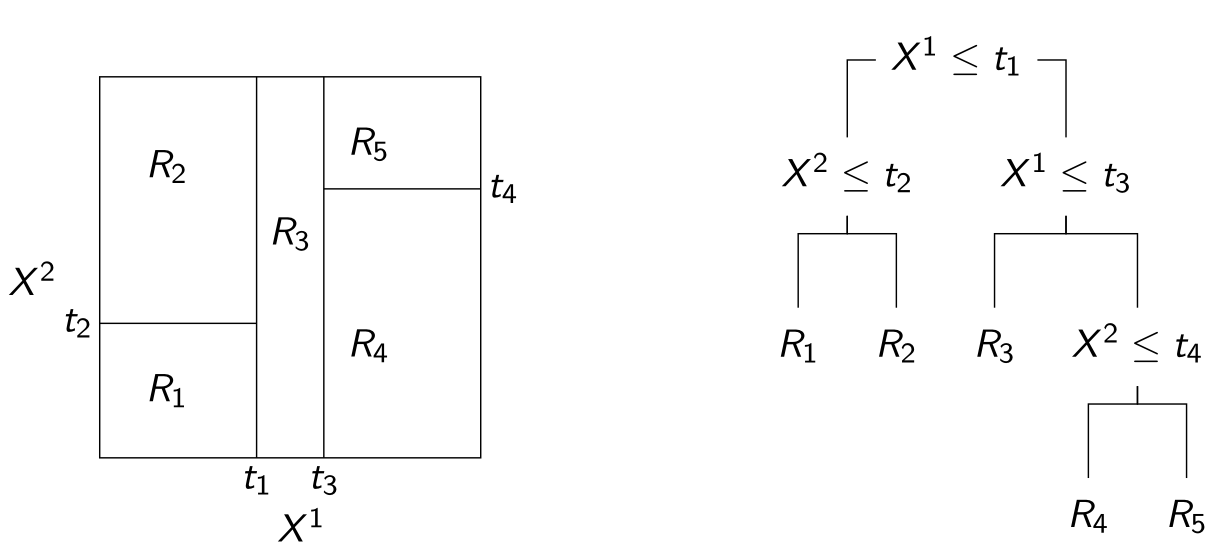
\includegraphics[width=0.8\linewidth]{images/03_methode/partition_cart}
	\caption{Schéma du partitionnement de l'espace des covariable par CART \cite{fischer2026}.}
	\label{fig:partitioncart}
\end{figure}

De manière plus formelle, on dispose d'un échantillon $\mathcal{D}_n = \{(X_1,Y_1),\dots,(X_n,Y_n)\}$ de couples indépendants et de même loi que $(X,Y)$, où $X = (X^{(1)},\dots,X^{(d)}) \in \mathbb{R}^d$ et $Y \in \mathbb{R}$. L'objectif est d'estimer la fonction de régression $f(x) = \mathbb{E}[Y \mid X = x]$. \\

\paragraph{Partitionnement et critère de coupure}
Un arbre partitionne récursivement l'espace des variables $\mathbb{R}^d$ en rectangles, chaque rectangle correspondant à un noeud de l'arbre. Soit $\mathcal{D}$ l'échantillon utilisé pour construire l'arbre, $R \subseteq \mathbb{R}^d$ un noeud et $n_R = \sum_{i}^n \mathds{1}_{\{X_i \in R\}}$ le nombre d'observations de $\mathcal{D}$ qui tombent dans $R$.\\

Une coupure est un couple $(j,t) \in \{1,\dots,d\} \times \mathbb{R}$, avec $j \in d$ la variable et $t \in \mathbb{R}$ le seuil de coupure. Elle partitionne le noeud $R$ en deux noeuds fils $R_1 (j,t)$ et $R_2(j,t)$ :
\[
R_1(j,t) = \{x \in R : x_j < t\}
\qquad\text{et}\qquad
R_2(j,t) = \{x \in R : x_j \ge t\},
\]
d'effectifs respectifs $n_1(j,t) = n_{R_1(j,t)}$ et $n_2(j,t) = n_{R_2(j,t)}$, avec $n_1(j,t) + n_2(j,t) = n_R$. 


On souhaite trouver une manière de partitionner les variables telle que les deux nouvelles régions $R_1 (j, t)$ et $R_2(j, t)$ issues de cette partition soient les plus homogènes possibles. Cela revient à, dans le cas de la régression, minimiser la variance de chaque noeud $R$ (critère d'impureté) :

\begin{equation}\label{eq:variance}
	V(R) = \frac{1}{n_R} \sum_{i : X_i \in R} \bigl(Y_i - \overline{Y}_R\bigr)^2
	\qquad\text{où}\qquad
	\overline{Y}_R = \frac{1}{n_R} \sum_{i : X_i \in R} Y_i .
\end{equation}

La qualité d'une coupure $(j,t)$ admissible est mesurée par la diminution d'impureté qu'elle produit, ou gain d'information (Information Gain, IG) :
\begin{equation}\label{eq:gain}
	\text{IG}_R(j,t) = V(R)
	- \frac{n_1(j,t)}{n_R}\, V\bigl(R_1(j,t)\bigr)
	- \frac{n_2(j,t)}{n_R}\, V\bigl(R_2(j,t)\bigr).
\end{equation}

Les variances des fils sont pondérées par la proportion d'observations qu'ils
contiennent, de sorte que $	\text{IG}_R(j,t) \ge 0$ (décomposition de la variance
totale en variances intra- et inter-groupes). La meilleure coupure parmi un
ensemble de variables candidates $\mathcal{M} \subseteq \{1,\dots,d\}$ est
\begin{equation}\label{eq:meilleure}
	(j^\star, t^\star) \in
	\text{argmax}_{j \in \mathcal{M},\; t \in \mathcal{T}_j(R)} 	\text{IG}_R(j,t).
\end{equation}

\paragraph{Prédiction d'un arbre}

Pour $x \in \mathbb{R}^d$, on note $R(x)$ la feuille de l'arbre $\hat f$ contenant $x$ et $n_{R(x)}$ le nombre de points de $\mathcal{D}_m$  qui y tombent. La prédiction de
l'arbre est la moyenne des réponses de cette feuille :
\begin{equation}
	\label{eq:arbre}
	\hat f(x) = \overline{Y}_{R(x)}
	= \frac{1}{n_{R(x)}}
	\sum_{(X_i,Y_i) \in \mathcal{D}_m} Y_i \, \mathds{1}_{\{X_i \in R(x)\}}
\end{equation}

\subsection{Forêt Aléatoire} 
\label{subsection:RF}
Une forêt aléatoire \cite{breiman2001} est une méthode de bagging consistant à tirer $B$ échantillons bootstrap à partir de $\mathcal{D}_n$, puis construire un arbre CART sur chacun d'eux et enfin agréger les prédictions des $B$ arbres. Les CART construits sont cependant légèremment différents : à chaque noeud, la meilleure coupure n'est pas cherchée parmi les $d$ variables, mais parmi un sous-ensemble de $p \le d$ variables tirées au hasard.

\paragraph{Construction de la forêt}
Pour $b = 1, \dots, B$, on tire avec remise un échantillon bootstrap $\mathcal{D}_m^{(b)}$ de taille $m$ dans $\mathcal{D}_n$, puis on construit un arbre $\hat f^{(b)}$ sur $\mathcal{D}_m^{(b)}$ par partitionnement récursif. À chaque noeud $R$, on tire uniformément et sans remise un ensemble $\mathcal{M} \subseteq \{1,\dots,d\}$ de $p$ variables, et on coupe $R$ selon la coupure $(j^\star, t^\star)$ définie par \eqref{eq:meilleure}. Le tirage de $\mathcal{M}$ est effectué indépendamment à chaque noeud. 

\paragraph{Prédiction de la forêt}
Pour chaque arbre $b \in [1, \ldots, B]$, la prédiction $\hat f^{(b)}(x)$ est donnée par \eqref{eq:arbre} (en remplaçant $\mathcal{D}_m$ par $\mathcal{D}_m^{(b)}$). La forêt prédit la moyenne des $B$ arbres :
\begin{equation}\label{eq:foret}
	\hat f_B(x) = \frac{1}{B} \sum_{b=1}^{B} \hat f^{(b)}(x).
\end{equation}

\paragraph{Hyperparamètres}
La construction de forêts aléatoires dépend donc de quatre hyperparamètres : 
\begin{itemize}
	\item $B$ le nombre d'arbres (\texttt{num.trees}),
	\item $m$ la taille des échantillons bootstrap (\texttt{sample.fraction}),
	\item $p$ le nombre de variables candidates pour chaque split (\texttt{mtry}),
	\item $n_{\min}$ l'effectif minimal des feuilles (\texttt{min.node.size})
\end{itemize}  
	
	
	
	
	
	
	
	
	
	
	
	
		



	
	\section{Protocole de validation croisée}
		\label{section:CV}
		\subsection{Prévention des fuites de données}
			Les données environnementales et biologiques présentent une structuration dépendante de la latitude : leurs propriétés statistiques varient donc selon la position dans l'espace. Les hypothèses de stationnarité d'ordre 1 (moyenne constante dans l'espace) et d'ordre 2 (structure de covariance invariante par translation, ne dépendant que de la distance entre points) ne sont donc pas respectées.
			
			De plus, lors des campagnes océanographiques, une onde acoustique est émise toutes les 3 à 4 secondes. La conséquence de cette proximité spatio-temporelle est la présence de pseudo-duplicatas dans le jeu de données. 
			
			Ces deux éléments, non-stationnarité spatiale et auto-corrélation, doivent être pris en compte lors de la construction du schéma de validation croisée, afin d'éviter toute fuite d'information entre les jeux d'entraînement et de validation (data leakage).
		\subsection{Validation croisée}
		
			% la description de la validation croisée est incomplète : il manque le pourquoi on fait ça !!
			La validation croisée est une méthode permettant consistant à diviser l'ensemble des données en $K$ sous-ensemble de taille à peu près identiques, appelés \textit{plis} (ou \textit{folds}). Un plis sert d'\textit{ensemble de validation} (ou \textit{ensemble test}) et les $K-1$ plis restants servent d'\textit{ensemble d'entraînement}. On obtient donc $K$ prédictions pour un même modèle. 
			
			Il existe différentes manières de sous-échantillonner les données pour construire les plis. Dans notre étude, nous avons testés différentes méthodes : validation croisée Monte-Carlo (Monte-Carlo Cross Validation, MC-CV) et la validation croisée par blocage spatio-temporel.
			\paragraph{Validation croisée Monte-Carlo (MC-CV)}
				Les analyses d'auto-correlation effectuée en section \ref{}
			\paragraph{Validation croisée par blocage spatio-temporel}
			
	\section{Ajustement des hyperparamètres}
	\section{Évaluation des performances}
		\subsection{Métriques et biais des prédictions}
	\section{Validation du modèle}
		\subsection{Sur-apprentissage et robustesse}
		\subsection{Recherche de raccourcis (shortcut learning)}
		\subsection{Domaine d'applicabilité}
	\section{Interprétation post-hoc}
		\subsection{Importance des variables (covariables corrélées)}
		\subsection{Analyse des résidus et suffisance des covariables}
	



















	\section{Schéma de validation}
	\section{Ajustement des hyperparamètres}
	\section{Validation}
	\subsection{validation des données}
	Le biais d'échantillonnage et le covariate shift portent sur les données : on peut les mesurer sans même avoir de modèle, en comparant les données d'entraînement à celles de la population cible ou de la production. C'est de la validation des données.
	\subsection{validation du protocole}
	La fuite de données porte sur le protocole : elle vient de la façon dont on a construit les variables, séparé les jeux d'entraînement et de test, ou choisi les informations disponibles au moment de prédire. La vérifier, c'est valider la conception de l'expérience.
	\subsection{validation du modèle}
	Valider un modèle, c'est établir qu'il est adapté à son usage prévu : que ses hypothèses tiennent, qu'il s'appuie sur des relations légitimes, qu'il reste fiable dans les conditions où il sera employé, et dans quel domaine il est applicable. Chercher à savoir à savoir si sa performance est fiable et si elle tiendra dans les conditions réelles.
	
	Le shortcut learning porte sur le modèle lui-même : il faut regarder ce qu'il a réellement appris, avec des outils d'interprétabilité ou des tests où l'on neutralise la variable suspecte. C'est de la validation du modèle au sens strict.
	
	Une fuite ou un biais d'échantillonnage dans les données est souvent ce qui rend possible un raccourci dans le modèle, et un décalage de distribution est ce qui fait apparaître ce raccourci en production.
	
	vérifier que le modèle n'overfit pas : robustesse au bruit
	vérifier que le modèle ne fais pas shortcut learning
	vérifier que le modèle est capable d'extrapoler 
	
	
	\section{Evaluation du modèle}
	vérifier que le modèle prédit de manière fiable et non biaisé
	
	\section{Interprétation post-hoc}
	\subsection{Importance des variables}
	\subsection{Source du biais} % mais ça en fait ca se fait avant sur la validation des données non ?
	\subsection{Suffisances des informations contenues par les covariables} % mais ça en fait ca se fait avant sur la validation des données non ?
	
	